\section{参数化曲线}\label{021}

【\ref{004}\nameref{004}】中提到过用隐函数来表示一些图像, 事实上,
我们还可以利用\textbf{参数化曲线} (parametric curve)
来比较方便表示一些较为复杂的图像. 还是以圆形位于原点的圆作为一个 trivial
例子, 【\ref{005}\nameref{005}】中我们简单地了解过极坐标, 不难发现, 圆周上的任意一点
\((x,y)\) 都可以写作 \((\cos\theta, \sin\theta)\); 于是, 我们可以将
\(\theta\) 视作圆的一个参数, 在 \(\theta\) 从 \(0\) 变为 \(2\pi\)
的过程中, 下面这一组函数便可绘出单位圆: \[
\begin{cases}
x(\theta)=\cos\theta\\
y(\theta)=\sin\theta
\end{cases}.
\]

如果希望求得这个函数某处的切线, 我们需要知道切线的斜率,
切线的斜率通常是通过 \(\frac{\mathrm{d}y}{\mathrm{d}x}\)求得的,
那么现在应该怎么办呢? 利用链式法则 (参见【\ref{013}\nameref{013}】) 可得 \[
\frac{\mathrm{d}y}{\mathrm{d}\theta}=\frac{\mathrm{d}y}{\mathrm{d}x}\frac{\mathrm{d}x}{\mathrm{d}\theta},
\] 所以我们可以先对前面的参数方程关于 \(\theta\) 求导,
然后利用下式得到其在某处的斜率 \[
\frac{\mathrm{d}y}{\mathrm{d}x}=\frac{\frac{\mathrm{d}y}{\mathrm{d}\theta}}{\frac{\mathrm{d}x}{\mathrm{d}\theta}}.
\]

\begin{newquote}
数学人震怒-1: 虽然不能这么理解, 但是为了记忆方便, 可以想象两个
\(\mathrm{d}\theta\) ``约掉了''.
\end{newquote}

\begin{tcolorbox}[size=fbox, breakable, enhanced jigsaw, title={弧长 (arc length)}]

弧长和圆的弧长其实关系并不大,
这个词在这里被用来描述一个函数图像的一段曲线长度.
初一看可能函数图像的一段曲线长度很难被描述, 但是要注意,
我们现在已经有了微积分这一非常有力的工具, 我们可以从``极限'',
``微元''这些角度去思考. 这种思路在物理和工程上尤为重要,
当我们试图找到变量之间的微分关系时.

\begin{tcolorbox}[size=fbox, breakable, enhanced jigsaw]
  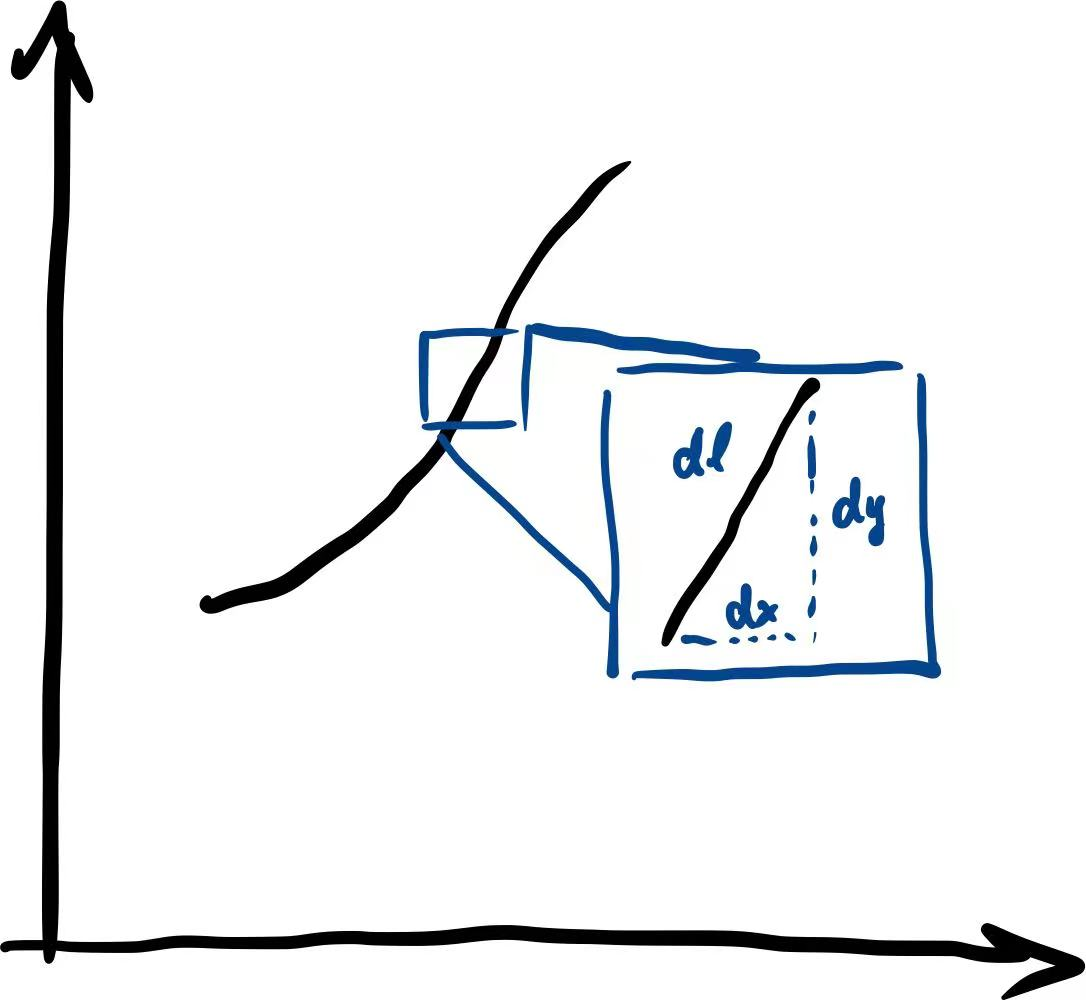
\includegraphics[width=0.3\textwidth]{img/image-20231108153210418.png}
\end{tcolorbox}

回到弧长, 当我们试图找到一段函数曲线的长度时, 我们可以先 zoom in (放大),
然后 focus on (观查) 其中非常小的一段, 当只关注其中非常小的一段时,
这一小段应该表现得足够线性 (如果不够线性, 那就是放大得还不够,
关注的区域不够小), 那么这一段弧长 \(\Delta l\)
应该可以利用勾股定理近似为 \(\sqrt{\Delta x^2+\Delta y^2}\),
然后取极限便有 \[
\boxed{\mathrm{d}l=\sqrt{\mathrm{d}x^2+\mathrm{d}y^2}}.
\] 当我们已知函数 \(y(x)\) 的情况下, 可以将上式改写为 \[
\mathrm{d}l=\sqrt{1+\left(\frac{\mathrm{d}y}{\mathrm{d}x}\right)^2}\mathrm{d}x.
\]

\begin{newquote}
数学人震怒-2: \textbf{相当于}把 \(\mathrm{d}x\) 提取出来了,
当然这么理解数学上是非常不严谨的, 但是物理和工程上 it just works.
\end{newquote}

于是, 在实际计算中, 若给定了函数 \(y(x)\),
其弧长便可以利用如下所示的积分计算 \[
l=\int\mathrm{d}l=\int\sqrt{1+\left(\frac{\mathrm{d}y}{\mathrm{d}x}\right)^2}\mathrm{d}x.
\]

\begin{newquote}
类似上式的思路在物理中很常见:

\begin{itemize}
\item
  比如对于质量分布不均匀的物体, 给定密度关于位置的函数 \(\rho(x,y,z)\),
  求质量, 利用 \(m=\rho V\) 便有:
  \(m=\int\mathrm{d}m=\int\rho(x,y,z)\mathrm{d}V=\iiint\rho(x,y,z)\mathrm{d}x\mathrm{d}y\mathrm{d}z\),
  这个积分的边界是这个物体的表面,
  所以最后一步的三重积分的上下限需要被非常小心地确定;
\item
  比如给定了电荷的分布, 求电场,
  利用\(E=\frac{Q}{4\pi\epsilon_0 r^2}\)有:
  \(\mathrm{d}E=\frac{1}{4\pi\epsilon_0}\frac{\mathrm{d}Q}{r^2}=\frac{1}{4\pi\epsilon_0}\frac{\rho}{r^2}\mathrm{d}V=\cdots\).
  当然, 严格来说这会是一个向量的积分, 暂时就不具体讲了.
\item
  \ldots{}
\end{itemize}

总而言之, 先从比较通常的情况 (质量均匀分布/点电荷/\ldots)
的变量关系出发, 然后一步步抽丝剥茧地将微元变为可以积分的变量为止
(\(\mathrm{d}m\Rightarrow \mathrm{d}V\Rightarrow\mathrm{d}x\mathrm{d}y\mathrm{d}z\))
.
\end{newquote}

那么如果给定的形式是一个参数化曲线呢? 例如, 已知 \(\{x(t),y(t)\}\),
那么可以先对 \(x(t)\) 和 \(y(t)\) 先分辨关于 \(t\) 求导, 得到
\(\mathrm{d}x\) 和 \(\mathrm{d}y\) 与 \(\mathrm{d}t\) 之间的微分关系,
然后弧长的微元便可以写作 \[
\mathrm{d}l=\sqrt{\left(\frac{\mathrm{d}x}{\mathrm{d}t}\right)^2+\left(\frac{\mathrm{d}y}{\mathrm{d}t}\right)^2}\mathrm{d}t.
\] 对其积分便可得到弧长.
\end{tcolorbox}